\documentclass[11pt,a4paper]{report}

% ---------------------------------------------------------------------------
% Packages
% ---------------------------------------------------------------------------
\usepackage[margin=1in]{geometry}
\usepackage{graphicx}
\usepackage{booktabs}
\usepackage{array}
\usepackage{xcolor}
\usepackage{hyperref}
\usepackage{titlesec}
\usepackage{fancyhdr}
\usepackage{enumitem}
\usepackage{caption}
\usepackage{float}
\usepackage{listings}
\usepackage{longtable}
\usepackage{amssymb}
\usepackage{tocloft}

% ---------------------------------------------------------------------------
% Colors
% ---------------------------------------------------------------------------
\definecolor{navy}{RGB}{44,92,138}
\definecolor{rust}{RGB}{166,93,30}
\definecolor{codebg}{RGB}{245,245,245}
\definecolor{codeframe}{RGB}{210,210,210}

% ---------------------------------------------------------------------------
% Section styling
% ---------------------------------------------------------------------------
\titleformat{\chapter}[display]
  {\normalfont\huge\bfseries\color{navy}}
  {\chaptertitlename\ \thechapter}{20pt}{\Huge}
\titleformat{\section}
  {\normalfont\Large\bfseries\color{navy}}{\thesection}{1em}{}
\titleformat{\subsection}
  {\normalfont\large\bfseries\color{navy!80!black}}{\thesubsection}{1em}{}

\pagestyle{fancy}
\fancyhf{}
\fancyhead[L]{\small\textit{Smart Inventory Command Center}}
\fancyhead[R]{\small\thepage}
\renewcommand{\headrulewidth}{0.4pt}

\hypersetup{
  colorlinks=true,
  linkcolor=navy,
  citecolor=navy,
  urlcolor=rust,
  pdftitle={Smart Inventory Command Center - Technical Report},
  pdfauthor={NovaLog Distribution Analytics}
}

\lstset{
  backgroundcolor=\color{codebg},
  rulecolor=\color{codeframe},
  frame=single,
  basicstyle=\ttfamily\footnotesize,
  breaklines=true,
  columns=fullflexible,
  keywordstyle=\color{navy}\bfseries,
  commentstyle=\color{gray}\itshape,
  stringstyle=\color{rust},
  showstringspaces=false,
}
\lstdefinelanguage{DAX}{
  keywords={CALCULATE, SUM, SUMX, AVERAGE, AVERAGEX, DIVIDE, FILTER, ALL, VAR, RETURN, TOTALYTD, SAMEPERIODLASTYEAR, DATEADD, DATESINPERIOD, DISTINCTCOUNT, COUNTROWS, SWITCH, TRUE, ISBLANK, FORMAT, MIN, MAX},
  sensitive=false,
  morecomment=[l]{//},
}

\setlength{\cftbeforechapskip}{8pt}

\begin{document}

% ===========================================================================
% Title page
% ===========================================================================
\begin{titlepage}
\centering
\vspace*{2cm}

{\Huge\bfseries\color{navy} Smart Inventory Command Center}\\[0.6cm]
{\Large A Supply Chain Analytics Platform for NovaLog Distribution}\\[1.5cm]

\rule{0.6\textwidth}{0.6pt}\\[0.5cm]
{\large Technical Report \& Architecture Documentation}\\[0.3cm]
{\normalsize End-to-end data pipeline: synthetic data generation, SQLite,\\
SQL analysis, Python/Pandas analytics, and Power BI}\\[1.5cm]
\rule{0.6\textwidth}{0.6pt}\\[2cm]

\begin{tabular}{rl}
\textbf{Company (fictional):} & NovaLog Distribution -- e-commerce logistics \\[4pt]
\textbf{Scale:} & 3 warehouses, 50 suppliers, 5{,}000 products, $\sim$100{,}000 orders \\[4pt]
\textbf{Tech stack:} & SQL (SQLite), Python, Pandas, NumPy, Matplotlib, Power BI \\[4pt]
\textbf{Repository:} & \texttt{smart-inventory-command-center} \\[4pt]
\end{tabular}

\vfill

{\normalsize Prepared as a portfolio project for Supply Chain / Logistics / BI\\
Data Analyst apprenticeship applications.}\\[0.5cm]
{\normalsize \today}

\end{titlepage}

\tableofcontents
\listoffigures
\clearpage

% ===========================================================================
\chapter{Executive Summary}
% ===========================================================================

This project builds a complete analytics platform for a fictional
e-commerce logistics company, \textbf{NovaLog Distribution}, spanning the
full path from synthetic data generation through SQL analysis, Python/Pandas
deep-dive analytics, and a Power BI-ready star schema. It is built in seven
numbered phases, each independently documented, tested, and committed.

\begin{table}[H]
\centering
\caption{Headline results (regenerated live by the pipeline)}
\begin{tabular}{lr}
\toprule
\textbf{Metric} & \textbf{Value} \\
\midrule
Delivered revenue & \$51.6M \\
Gross margin & \$13.9M (27.0\%) \\
Inventory value at cost & \$8.0M \\
Capital in dead stock (sales-velocity definition) & \$3.4M (42.0\% of inventory) \\
Suppliers flagged High Risk & 4 of 50 \\
Supplier scorecard validity & $r = 0.838$ vs.\ hidden ground truth \\
Top warehouse by revenue & Central DC (\$21.98M, 6.84\% return rate) \\
\bottomrule
\end{tabular}
\end{table}

\section*{What this report demonstrates}
\begin{itemize}[leftmargin=1.4em]
  \item A normalized, constraint-enforced relational data model, and a
        separately-modeled Power BI star schema derived from it --
        understanding \emph{why} these are different is itself a core BI
        skill.
  \item Statistically calibrated synthetic data generation (Section
        \ref{sec:data-gen}), grounded in published benchmarks rather than
        naive uniform randomness.
  \item Six SQL queries directly answering the project's business
        questions, plus a Python/Pandas layer for the analysis SQL is
        poorly suited to (time trends, cohort-style aging, composite
        scoring).
  \item Complete DAX measure library and Power BI build specification.
  \item \textbf{Two real, non-trivial bugs found and fixed} during
        development (Chapter \ref{ch:postmortem}) -- both passed every
        single-table validation check and were only caught by reasoning
        about relationships \emph{between} tables. This chapter is
        deliberately included in full: catching your own mistakes and
        explaining the fix is a stronger signal of analytical skill than a
        report claiming everything worked first time.
\end{itemize}

% ===========================================================================
\chapter{Architecture \& Pipeline}
% ===========================================================================

\section{Pipeline overview}

The system is organized as six sequential phases, each with a single Python
entry point and its own automatic validation step. Figure
\ref{fig:architecture} shows how they connect.

\begin{figure}[H]
\centering
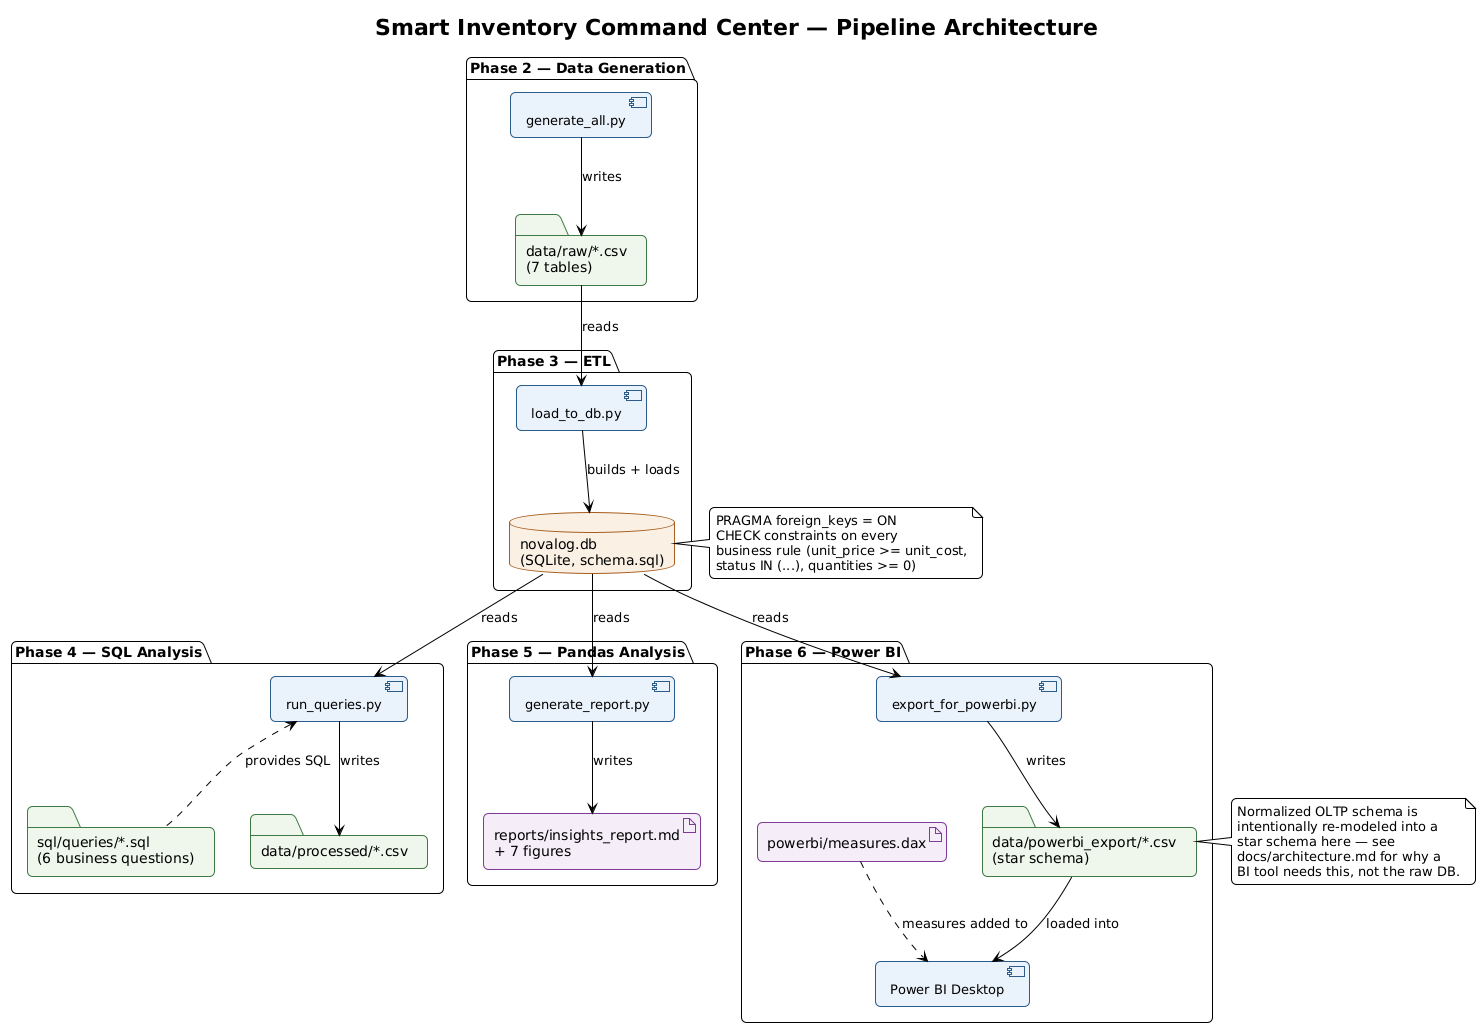
\includegraphics[width=\textwidth]{../diagrams/architecture.png}
\caption{Pipeline architecture: each phase reads the previous phase's
output and validates its own before handing off.}
\label{fig:architecture}
\end{figure}

\begin{table}[H]
\centering
\caption{Phase-to-entry-point mapping}
\begin{tabular}{clp{7.3cm}}
\toprule
\textbf{Phase} & \textbf{Entry point} & \textbf{Produces} \\
\midrule
2 & \texttt{src.data\_generation.generate\_all} & 7 CSVs in \texttt{data/raw/}, validated by 22 checks \\
3 & \texttt{src.etl.load\_to\_db} & \texttt{novalog.db} (SQLite), zero FK violations \\
4 & \texttt{src.analysis.run\_queries} & 6 business-question results in \texttt{data/processed/} \\
5 & \texttt{src.analysis.generate\_report} & \texttt{reports/insights\_report.md} + 7 figures \\
6 & \texttt{src.etl.export\_for\_powerbi} & Star schema in \texttt{data/powerbi\_export/}, validated by 13 checks \\
\bottomrule
\end{tabular}
\end{table}

Every stage is idempotent and fully reproducible: the same random seed
(\texttt{config.RANDOM\_SEED}) produces byte-identical output on every run,
which matters because this report's own figures and screenshots must match
what anyone re-running the pipeline sees.

\section{Execution sequence}

Figure \ref{fig:sequence} traces a complete pipeline run end to end,
including the validation step embedded in each stage.

\begin{figure}[H]
\centering
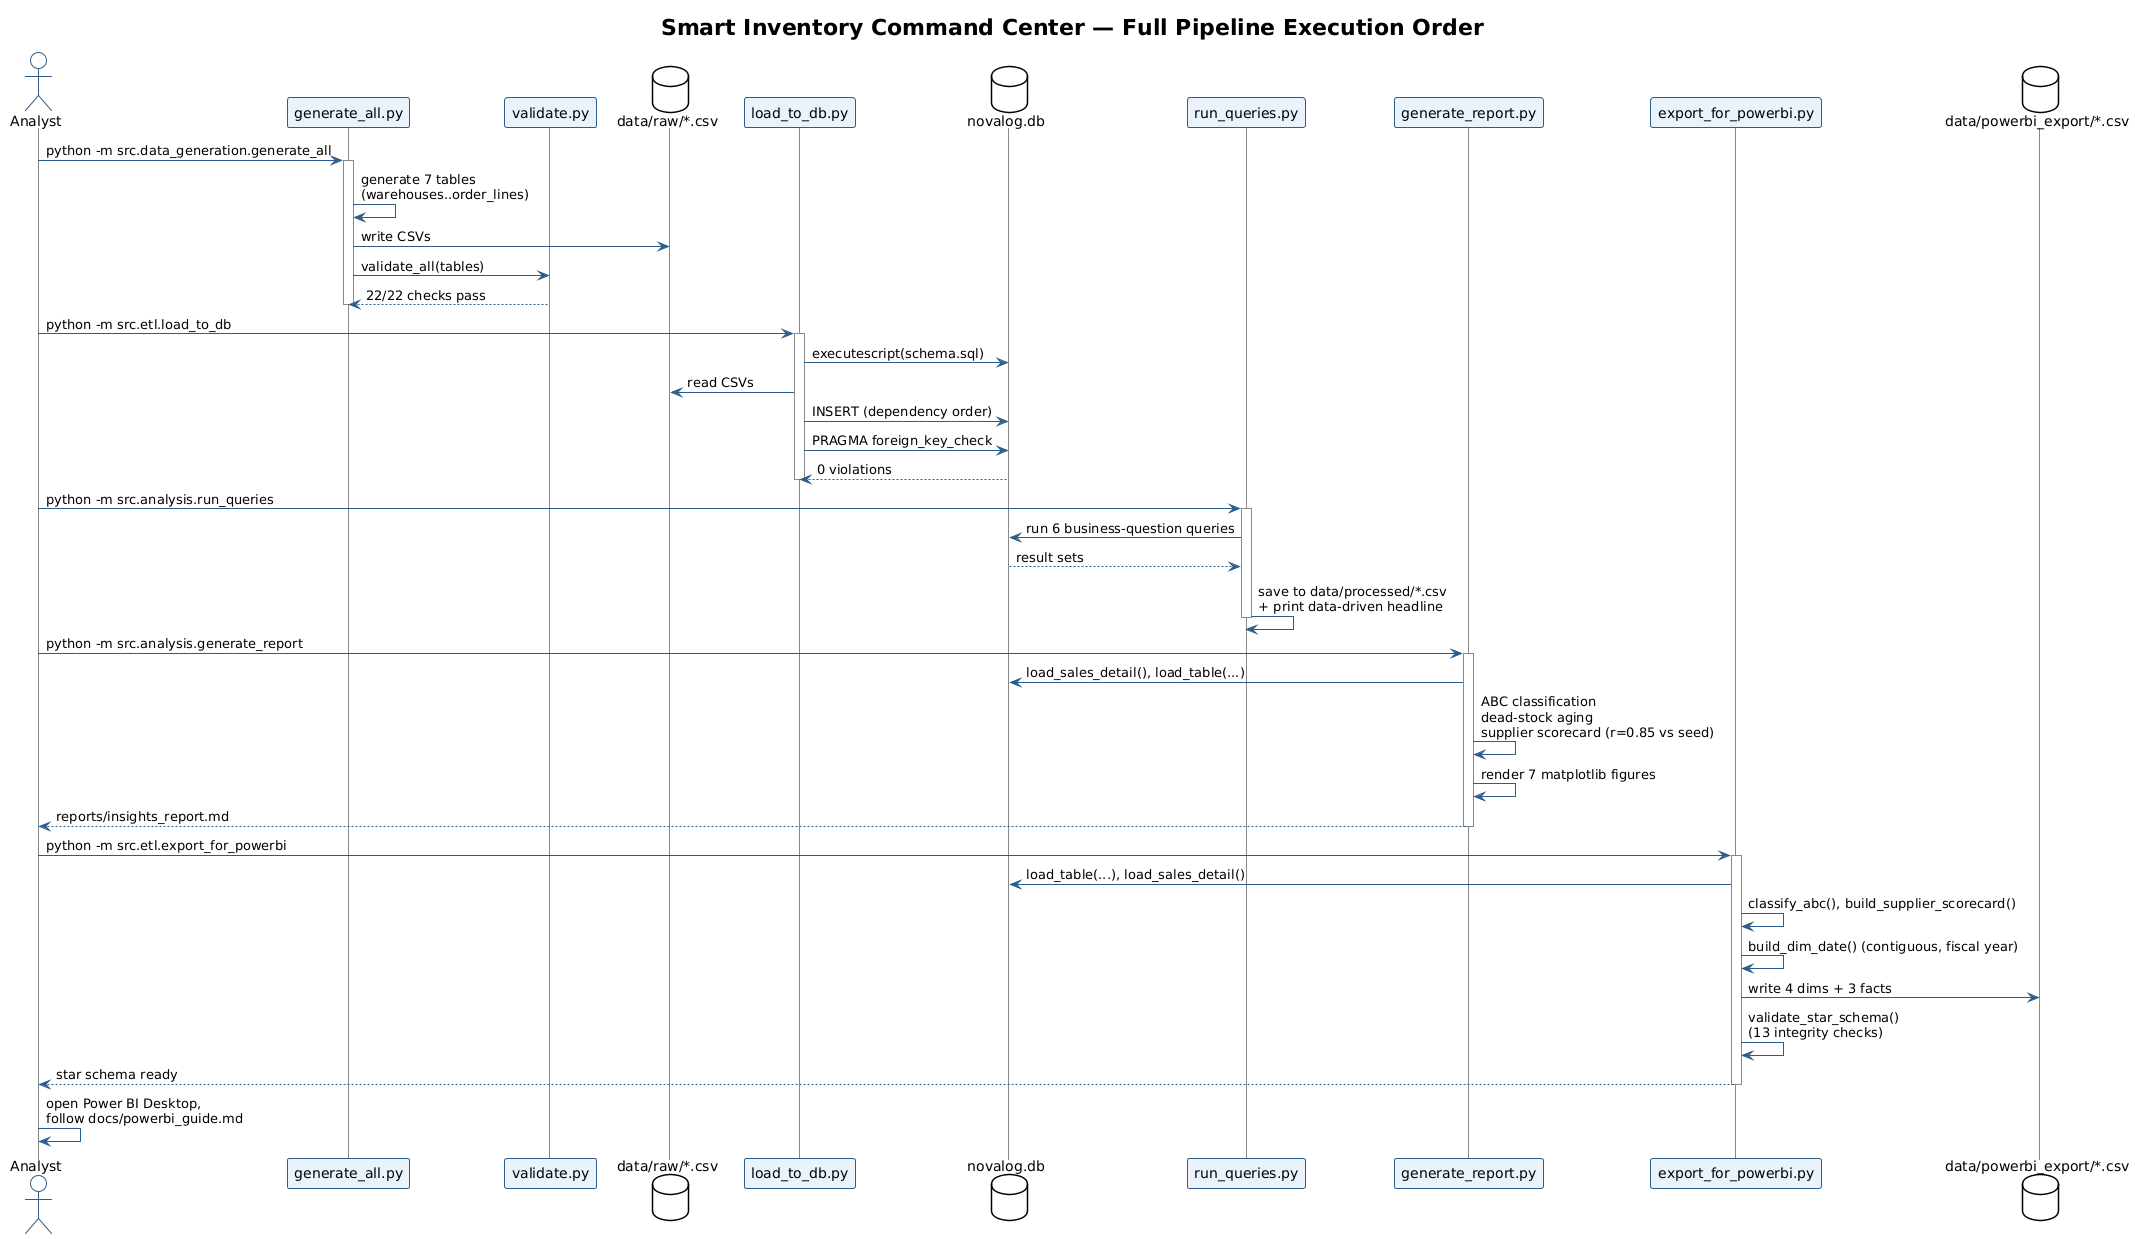
\includegraphics[width=\textwidth]{../diagrams/pipeline_sequence.png}
\caption{Full pipeline execution order, including each stage's internal
validation call.}
\label{fig:sequence}
\end{figure}

% ===========================================================================
\chapter{Data Model}
% ===========================================================================

\section{Entity-relationship design}

The database is deliberately modeled as a normalized OLTP-style schema
rather than a pre-built star schema. Real operational systems hand you
transactional tables, not a warehouse -- modeling it this way lets the
project demonstrate both halves of the skill: designing a transactional
model, then separately transforming it into an analysis-ready star schema
for Power BI (Chapter \ref{ch:powerbi}).

\begin{figure}[H]
\centering
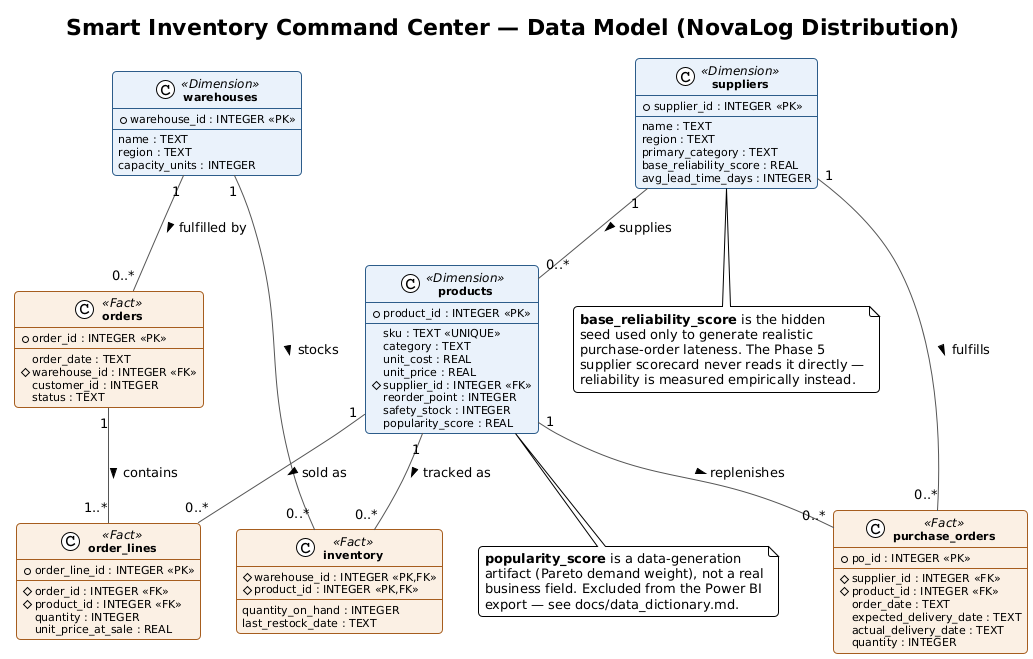
\includegraphics[width=\textwidth]{../diagrams/data_model.png}
\caption{Data model as a UML class diagram. Dimension tables (blue) hold
descriptive attributes; fact tables (orange) hold transactional events.
Stereotypes mark primary and foreign keys.}
\label{fig:data-model}
\end{figure}

\section{Design decisions}

\begin{description}[leftmargin=1.4em, style=nextline]
  \item[\texttt{unit\_price\_at\_sale} stored on \texttt{order\_lines}, separate
    from \texttt{products.unit\_price}.] Prices drift over a two-year window;
    storing the historical sale price is what real transactional systems do,
    and it matters for accurate revenue reporting when catalog prices
    change after a sale.

  \item[\texttt{suppliers.primary\_category} (schema addition).] Not part
    of the original design -- added so products can be assigned to
    suppliers who plausibly sell that category of product, rather than an
    arbitrary pairing (an electronics wholesaler is unlikely to also ship
    groceries).

  \item[\texttt{products.popularity\_score} (simulation-only field).] Does
    not exist in a real operational system. It is the internal Pareto/Zipf
    demand weight the generator uses to concentrate sales realistically
    (Section \ref{sec:data-gen}). It is explicitly excluded from the Power
    BI export (Chapter \ref{ch:powerbi}) so it can never be mistaken for a
    real business attribute.

  \item[One supplier per product, not a many-to-many bridge table.] A
    \texttt{product\_suppliers} bridge table would model dual-sourcing, but
    none of the six business questions this project answers require it. A
    schema exactly as complex as the questions it serves is a deliberate
    choice, not an oversight -- documented here as an explicit extension
    point (Chapter \ref{ch:future}) rather than built speculatively.

  \item[Foreign keys and CHECK constraints enforced at the database level,
    not just in application code.] \texttt{sql/schema.sql} declares
    \texttt{PRAGMA foreign\_keys = ON}, every relationship as a
    \texttt{FOREIGN KEY}, and business rules as \texttt{CHECK} constraints
    (e.g.\ \texttt{unit\_price >= unit\_cost}, \texttt{status IN (\ldots)}).
    SQLite disables FK enforcement by default -- easy to forget, and it
    would silently let invalid data in if left off.

  \item[Dates stored as ISO-8601 TEXT.] SQLite has no native date type;
    \texttt{YYYY-MM-DD} text sorts correctly under plain string comparison
    and works directly with SQLite's \texttt{date()} / \texttt{julianday()}
    functions.
\end{description}

\section{Schema at a glance}

\begin{table}[H]
\centering
\caption{Table sizes at full generation scale}
\begin{tabular}{lr}
\toprule
\textbf{Table} & \textbf{Rows} \\
\midrule
warehouses & 3 \\
suppliers & 50 \\
products & 5{,}000 \\
inventory & 15{,}000 \\
purchase\_orders & $\sim$25{,}000 \\
orders & 100{,}000 \\
order\_lines & $\sim$190{,}000 \\
\bottomrule
\end{tabular}
\end{table}

% ===========================================================================
\chapter{Data Generation Methodology}
\label{sec:data-gen}
% ===========================================================================

\section{Reference-informed simulation}

Rather than generating data with naive uniform randomness, every
distribution is calibrated against published statistics from the
\textbf{DataCo Smart Supply Chain for Big Data Analysis} dataset (Kaggle,
$\sim$18{,}000 orders) -- not imported directly (it requires authenticated
API access unavailable in this environment), but used as calibration
targets for this project's own generator.

\begin{table}[H]
\centering
\caption{Calibration targets and what drives them in the generator}
\begin{tabular}{p{5.2cm}p{7.8cm}}
\toprule
\textbf{Calibrated pattern} & \textbf{Implementation} \\
\midrule
$\sim$90\% on-time delivery rate &
  Two-stage model: Bernoulli gate for \emph{is this PO late} (probability
  driven by supplier reliability), then exponential delay magnitude if
  late. Collapsing these into one continuous noise term was the exact
  mistake caught in the first generation run (Section \ref{sec:bug1-precursor}). \\
Supplier reliability is skewed, not uniform &
  \texttt{Beta(8, 2)} distribution: mean $\approx 0.8$ with a long left
  tail, mirroring real supplier networks where most vendors are dependable
  and a minority are chronically unreliable. \\
Revenue concentration (Pareto/80-20) &
  Zipf-distributed \texttt{popularity\_score} drives product selection in
  \texttt{order\_lines.py}; observed result is 8.1\% of SKUs generating
  80.0\% of revenue. \\
Seasonal order volume &
  Month-level weights peaking in Nov/Dec (holiday e-commerce), dipping
  mid-year -- fully vectorized date sampling, no per-row Python loop. \\
Order status mix &
  90\% Delivered / 3\% Cancelled / 7\% Returned, consistent with typical
  e-commerce norms. \\
\bottomrule
\end{tabular}
\end{table}

\section{Demand-derived inventory thresholds}

Following the bug fix described in Chapter \ref{ch:postmortem},
\texttt{reorder\_point} and \texttt{safety\_stock} are computed from actual
simulated demand rather than an arbitrary popularity-rank formula:

\begin{lstlisting}[language=Python, caption=Demand-derived stock thresholds (src/data\_generation/products.py)]
daily_demand   = expected_annual_units / 365 / N_WAREHOUSES
lead_time_demand = daily_demand * supplier_avg_lead_time_days
safety_stock   = max(lead_time_demand * SAFETY_STOCK_FACTOR, MIN_SAFETY_STOCK)
reorder_point  = lead_time_demand + safety_stock
\end{lstlisting}

\texttt{SAFETY\_STOCK\_FACTOR} and \texttt{MIN\_SAFETY\_STOCK} are centralized
in \texttt{config.py} so \texttt{products.py} (which sets the thresholds) and
\texttt{order\_lines.py} (which generates the demand that should satisfy
them) cannot silently drift apart.

\section{Independent random streams}

Every generator module draws from a named, independent random stream rather
than a single shared seed:

\begin{lstlisting}[language=Python, caption=Named independent streams (src/data\_generation/utils.py)]
def get_rng(stream: str, seed: int = config.RANDOM_SEED):
    entropy = [seed, zlib.crc32(stream.encode("utf-8"))]
    return np.random.default_rng(np.random.SeedSequence(entropy))
\end{lstlisting}

This is what fixed the second bug in Chapter \ref{ch:postmortem} --
reproducibility (same stream name always yields the same sequence) and
statistical independence (different names yield decorrelated sequences)
are both preserved simultaneously.

\section{Validation}

\texttt{src/data\_generation/validate.py} runs 22 automatic checks after
every generation run: row counts, referential integrity across all seven
tables, positivity constraints (no negative prices or quantities), and
calibration-band checks (on-time rate, stockout share, dead-stock share,
revenue concentration all fall within realistic ranges). All 22 currently
pass. Critically -- and this is the central lesson of Chapter
\ref{ch:postmortem} -- every one of these checks operates on a single table
at a time, which is precisely why they could not catch either bug described
there.

% ===========================================================================
\chapter{SQL Analysis: The Six Business Questions}
% ===========================================================================

Each business question from the project brief has its own file under
\texttt{sql/queries/}, executed by \texttt{src/analysis/run\_queries.py},
which prints a data-driven headline for each and saves the full result to
\texttt{data/processed/}.

\section{Which warehouse performs best?}

\begin{table}[H]
\centering
\caption{Warehouse performance -- revenue and order quality side by side}
\begin{tabular}{lrrrr}
\toprule
\textbf{Warehouse} & \textbf{Orders} & \textbf{Revenue} & \textbf{Avg.\ Order} & \textbf{Return \%} \\
\midrule
Central DC & 38{,}372 & \$21.98M & \$572.84 & 6.84\% \\
East Coast DC & 32{,}344 & \$18.51M & \$572.37 & 6.89\% \\
West Coast DC & 29{,}284 & \$16.81M & \$574.09 & 7.05\% \\
\bottomrule
\end{tabular}
\end{table}

Central DC leads on revenue \emph{and} carries the lowest return rate,
making it the clear top performer here -- but the query deliberately
reports both dimensions together rather than ranking by revenue alone,
since a large facility with a high return rate would be a false positive
for "best."

\subsection*{Key design choice}
Revenue is aggregated once per order in a CTE \emph{before} joining to
warehouses. Joining \texttt{order\_lines} directly to warehouses would
multiply each order's status flag by however many line items it has,
silently inflating the return/cancellation rate calculations -- a subtle
join-fanout bug that a naive query would not surface as an error, only as
a quietly wrong number.

\section{Which products generate the most revenue?}

Top SKU: \textbf{SPO-02112} (Sports \& Outdoors) -- \$12.08M from 39{,}234
units sold. The query reports margin alongside revenue, since a
high-revenue, low-margin product may matter less to the business than it
first appears.

\section{Which SKUs are at risk of stockout?}

Reported at the (product, warehouse) grain, not aggregated company-wide --
stockout is a per-location operational problem. A product can look healthy
in total stock while one specific warehouse is critically low; aggregating
across warehouses first would hide exactly that case.

\section{Which suppliers are unreliable?}

Least reliable: \textbf{Williams and Sons} -- 90.96\% late across 706
purchase orders. This query deliberately does \emph{not} read
\texttt{suppliers.base\_reliability\_score}: that column is a
data-generation seed a real analyst would never have access to. Reliability
here is computed purely from observed \texttt{purchase\_orders} history
(actual vs.\ expected delivery dates).

\section{How much inventory value is tied up in dead stock?}

\$2.24M under the SQL definition (quantity\_on\_hand $\geq$ 4$\times$
safety\_stock), valued at \texttt{unit\_cost} rather than
\texttt{unit\_price} -- dead stock represents capital already spent
acquiring inventory, not lost future revenue. Note this differs from the
\$3.4M figure in Chapter \ref{ch:pandas}, which uses a stricter Pandas
definition requiring \emph{zero sales in 90 days} in addition to the stock
threshold; the discrepancy is intentional and discussed there.

\section{Which products should be reordered?}

Sizes a concrete \texttt{recommended\_order\_quantity} (safety stock + 30
days of actual sales velocity, minus what's on hand) at the (product,
warehouse) grain -- a flag with no quantity attached is not actionable for
a buyer. Largest current recommendation: 1{,}238 units of SPO-02112.

\subsection*{A bug caught during development}
This query originally aggregated stock across all three warehouses before
comparing it to \texttt{reorder\_point} and returned \textbf{zero rows}.
The cause: \texttt{reorder\_point} is a per-warehouse threshold (that is
how \texttt{inventory.py} used it during data generation), so a company-wide
total is roughly 3$\times$ larger and almost never dips below a
single-warehouse threshold. Fixed by moving the query to the (product,
warehouse) grain, matching \texttt{stockout\_risk.sql}, and covered going
forward by \texttt{tests/test\_analysis.py}.

% ===========================================================================
\chapter{Python/Pandas Deep-Dive Analysis}
\label{ch:pandas}
% ===========================================================================

SQL answers the six core business questions well, but is poorly suited to
time-series trends, cohort-style aging, and composite scoring --
\texttt{src/analysis/} covers exactly that gap, orchestrated by
\texttt{generate\_report.py} into \texttt{reports/insights\_report.md} and
seven Matplotlib figures.

\section{ABC revenue classification}

8.1\% of SKUs (class A, 402 products) generate 80.0\% of revenue -- a
textbook Pareto distribution (Figure \ref{fig:abc}). Class A items justify
tight inventory control and priority warehouse space; class C items (61\%
of SKUs for 5.0\% of revenue) should be managed with minimal overhead.

\begin{figure}[H]
\centering
\includegraphics[width=0.85\textwidth]{../../reports/figures/abc_pareto.png}
\caption{Revenue concentration -- cumulative share of revenue by cumulative share of SKUs.}
\label{fig:abc}
\end{figure}

\section{Inventory turnover by category}

Sports \& Outdoors turns over fastest at 4.51$\times$/year (81 days of
supply); Apparel is slowest at 1.40$\times$ (261 days of supply). Slow
turnover is where working capital sits idle, and is the first place to
target for order-quantity reductions.

\emph{Methodology caveat:} this dataset holds a single current inventory
snapshot rather than a historical series, so turnover is computed against
ending inventory rather than true average inventory. Cross-category
comparison is valid; absolute values are approximate.

\section{Supplier reliability scorecard}

The composite score weights on-time rate (50\%), average delay severity
(30\%), and delay consistency (20\%). Consistency earns its own weight
because a predictably-late supplier can be planned around; an erratic one
cannot. Four suppliers fall into the \textbf{High Risk} tier; the weakest,
Williams and Sons, has a composite score of 4.5/100.

\begin{figure}[H]
\centering
\includegraphics[width=0.85\textwidth]{../../reports/figures/supplier_risk.png}
\caption{Bottom 15 suppliers by composite reliability score, colored by risk tier.}
\label{fig:supplier-risk}
\end{figure}

\subsection*{Methodology self-validation}
The scorecard is built \emph{purely} from observed purchase-order delivery
behavior -- it never reads \texttt{suppliers.base\_reliability\_score}, the
hidden seed value the data generator used to produce realistic lateness
patterns. Correlating the finished scorecard against that hidden seed
\emph{afterward}, purely as a check, gives $r = 0.838$: strong evidence the
scoring methodology recovers genuine underlying reliability signal rather
than fitting noise in the observed data. This is the single strongest piece
of methodological validation in the project, precisely because the ground
truth was never available to the scoring function itself.

\section{Dead stock, slow-moving, and overstocked}

\$3.4M (42.0\% of total inventory value) sits in positions with
\textbf{zero sales in the last 90 days} and stock at 2$\times$ safety level
or above. The classification deliberately distinguishes:

\begin{itemize}[leftmargin=1.4em]
  \item \textbf{Overstocked} -- high stock, but still selling; will clear on its own.
  \item \textbf{Dead} -- stranded capital with no recent sales; needs
    markdown, liquidation, or write-off.
\end{itemize}

A stock-level-only view (as used by the SQL query in Chapter 4) cannot
distinguish these -- which is exactly why this figure (\$3.4M) differs
from the SQL query's \$2.24M: the two use different, equally valid,
definitions of "dead" for different purposes. Electronics carries the most
at-risk capital at \$1.5M.

\begin{figure}[H]
\centering
\includegraphics[width=0.85\textwidth]{../../reports/figures/inventory_health_mix.png}
\caption{Inventory health mix: healthy, overstocked, and dead stock by category.}
\label{fig:inventory-health}
\end{figure}

\section{Recommended actions}

\begin{enumerate}[leftmargin=1.4em]
  \item Differentiate inventory policy by ABC class -- tighten review
    cycles on class A SKUs, reduce overhead on class C.
  \item Open supplier reviews with the 4 High Risk suppliers, starting
    with Williams and Sons; increase safety stock where dual-sourcing
    isn't viable.
  \item Run a liquidation review on dead stock, prioritizing Electronics.
  \item Reduce order quantities in slow-turning categories so the problem
    doesn't regenerate after liquidation.
\end{enumerate}

% ===========================================================================
\chapter{Power BI Dashboard}
\label{ch:powerbi}
% ===========================================================================

\section{Why no \texttt{.pbix} file}

\texttt{.pbix} is a proprietary, Windows-only binary format with no
supported programmatic authoring path -- it cannot be generated from
Python, and any tool claiming to do so would produce a file that does not
reliably open. What \emph{is} prepared here is everything that carries the
actual analytical substance: the dimensional model, the complete DAX
measure library, and a step-by-step build specification
(\texttt{docs/powerbi\_guide.md}). Assembling the report from these takes
roughly an hour in Power BI Desktop -- and means the finished report is
genuinely the reader's own work to defend in an interview, not a black box
they received.

\section{Star schema}

The normalized OLTP database (Chapter 3) is deliberately re-modeled into a
star schema for Power BI: 4 dimension tables and 3 fact tables, exported by
\texttt{src/etl/export\_for\_powerbi.py}.

\begin{table}[H]
\centering
\caption{Star schema exports}
\begin{tabular}{lrl}
\toprule
\textbf{Table} & \textbf{Rows} & \textbf{Notes} \\
\midrule
dim\_date & 731 & Contiguous, gap-free; required for DAX time intelligence \\
dim\_product & 5{,}000 & Enriched with ABC class; \texttt{popularity\_score} dropped \\
dim\_supplier & 50 & Enriched with risk tier; \texttt{base\_reliability\_score} dropped \\
dim\_warehouse & 3 & \\
fact\_sales & $\sim$171{,}000 & Excludes cancelled orders (no realized revenue) \\
fact\_inventory & 15{,}000 & \\
fact\_purchase\_orders & $\sim$25{,}000 & Lateness pre-derived (\texttt{is\_late}, \texttt{delay\_days}) \\
\bottomrule
\end{tabular}
\end{table}

\subsection*{Why a star schema at all, rather than pointing Power BI at the
normalized database}
DAX and Power BI's VertiPaq engine are built around one-to-many
dimension-to-fact filtering. Pointing a BI tool at a normalized model
instead forces bidirectional and snowflaked relationships, which are both
slower and -- more importantly -- create ambiguous filter propagation paths
that can silently return wrong numbers with no error message.

\subsection*{Why a dedicated \texttt{dim\_date} table}
Power BI's time-intelligence functions (\texttt{TOTALYTD},
\texttt{SAMEPERIODLASTYEAR}, \texttt{DATEADD}) require a contiguous,
gap-free date dimension explicitly marked as the model's date table.
Without one, these functions misbehave silently around any gap.

\subsection*{Generation artifacts are dropped, not carried forward}
\texttt{popularity\_score} and \texttt{base\_reliability\_score} were
internal inputs the synthetic data generator needed; a real analyst never
has them, and leaving them in the exported model would let the Power BI
analysis "cheat" by referencing values it should have no access to. Both
are explicitly stripped in the export step and checked for absence by an
automatic validation.

\section{Export validation}

Thirteen automatic checks run after every export: every foreign key in
every fact table resolves to its dimension, every dimension key is unique,
\texttt{dim\_date} is contiguous, and no generation-artifact column
survived. This matters because a broken relationship in Power BI does not
throw an error -- it silently drops rows or blanks out a visual, which is
far harder to diagnose than a crash.

\section{DAX measure library}

\texttt{powerbi/measures.dax} defines around 30 explicit measures (written
by hand, not Power BI's auto-generated implicit measures) across six
groups: sales \& profitability, order quality, time intelligence,
inventory, supplier performance, and ABC analysis. Two representative
examples:

\begin{lstlisting}[language=DAX, caption=Order count at the correct grain]
Order Count =
DISTINCTCOUNT ( fact_sales[order_id] )
// fact_sales is at order-LINE grain; COUNTROWS would count lines,
// not orders.
\end{lstlisting}

\begin{lstlisting}[language=DAX, caption=A measure that must not return 100\% inside its own filter]
Class A Revenue % =
DIVIDE (
    [Class A Revenue],
    CALCULATE ( [Total Revenue], ALL ( dim_product ) )
)
// ALL(dim_product) removes the product-level filter from the
// denominator so this compares against TOTAL revenue, not the
// already-filtered subset -- without it, this measure returns 100%
// inside any visual already filtered to class A.
\end{lstlisting}

\section{Report design}

The build guide specifies four pages: Executive Overview, Warehouse
Performance, Inventory Health, and Supplier Scorecard -- each with a
specific visual layout, and each deliberately designed so no single
misleading ranking (e.g., "biggest warehouse" or "highest revenue product")
stands without its quality counter-metric alongside it.

% ===========================================================================
\chapter{Engineering Postmortem: Two Bugs Caught}
\label{ch:postmortem}
% ===========================================================================

This chapter is included deliberately and in full. Both bugs below passed
every validation check written at the time they were introduced -- they
were not caught by more testing, but by a different \emph{kind} of
reasoning: checking a relationship between two tables rather than a
property of one table alone. That distinction is the actual lesson worth
taking from this project.

\section{Bug 1: Inventory thresholds disconnected from demand}

\subsection*{The bug}
The first version of \texttt{products.py} sized \texttt{safety\_stock} as:
\begin{lstlisting}[language=Python]
safety_stock = 20 + rank_percentile(popularity_score) * 480
\end{lstlisting}
a formula with no relationship to how much each SKU actually sells. The
consequence: the median SKU held roughly 260 units while selling
approximately 8 units per year.

\subsection*{How it was (almost) missed}
\label{sec:bug1-precursor}
Every Phase 2 validation check passed. The generation-time checks in
Chapter \ref{sec:data-gen} confirmed the intended proportions of
stockout-risk and dead-stock \emph{positions} (12\% and 10\% of inventory
rows respectively) -- and those proportions were, in fact, exactly
correct. In Phase 4's SQL analysis, the resulting \$1.04B total inventory
valuation and \$228M "dead stock" figure were sanity-checked by confirming
dead-stock positions held 4--8$\times$ their nominal safety stock level --
which they did, by construction. The check confirmed the data was
internally consistent with the (broken) rule that generated it, which is
not the same as confirming the rule was realistic.

\subsection*{What actually caught it}
Building the Phase 5 Pandas analysis required computing \textbf{inventory
turnover} -- annual cost of goods sold divided by inventory value. This is
the one metric that necessarily joins sales history against stock levels.
It returned 0.04$\times$, against a realistic retail range of 4--8$\times$.

\begin{table}[H]
\centering
\caption{Bug 1: before and after}
\begin{tabular}{lrr}
\toprule
\textbf{Metric} & \textbf{Before} & \textbf{After} \\
\midrule
Median units on hand & 260 & 14 \\
Portfolio inventory turnover & 0.04$\times$ & 2.13$\times$ \\
Total inventory value & \$1.04B & \$7.8M \\
Dead stock value & \$228M & \$1.9M \\
\bottomrule
\end{tabular}
\end{table}

\subsection*{The fix}
Replaced the arbitrary formula with demand-derived thresholds computed
from each product's actual expected sales velocity (Section
\ref{sec:data-gen}):
\begin{lstlisting}[language=Python]
lead_time_demand = daily_demand * supplier_lead_time_days
safety_stock     = lead_time_demand * SAFETY_STOCK_FACTOR
reorder_point    = lead_time_demand + safety_stock
\end{lstlisting}

\subsection*{Regression coverage added}
\texttt{tests/test\_data\_generation.py} now computes portfolio-level
inventory turnover directly from generated data and asserts it falls
within a realistic band -- a genuinely cross-table check that would have
caught the original bug immediately.

\section{Bug 2: RNG seed reuse silently correlated two independent tables}

\subsection*{The bug}
Every generator module called an unparameterized \texttt{get\_rng()}, which
returned \texttt{np.random.default\_rng(42)} -- literally the same random
stream in every module. NumPy draws categorical samples via inverse-CDF
transforms applied to an underlying uniform sequence. Since
\texttt{orders.py} (drawing each order's month) and \texttt{order\_lines.py}
(drawing each order's line count) both consumed their \emph{first} draw
from that identical stream, the two became perfectly rank-correlated: a
low uniform value produced both an early month \emph{and} a 1-line order; a
high value produced both a late month \emph{and} a 4-line order.

\subsection*{How it was (almost) missed}
Every marginal distribution was exactly correct: line counts followed the
specified 45/30/15/10 split, and order dates followed the intended seasonal
curve. Every single-table validation check passed, because there was
nothing wrong with either table considered alone.

\subsection*{What actually caught it}
Building the Phase 5 monthly revenue trend chart surfaced a suspicious
pattern: December 2025 revenue was roughly 2.4$\times$ December 2024, and
the entirety of 2025 trended visibly above 2024, despite the underlying
order-count seasonality being nearly identical year over year. Grouping
\texttt{lines-per-order} by calendar month exposed the mechanism precisely:
exactly 1.00 for every month of 2024, rising in a straight line to exactly
4.00 by December 2025.

\begin{table}[H]
\centering
\caption{Bug 2: lines per order by half-year (excerpt)}
\begin{tabular}{lr}
\toprule
\textbf{Period} & \textbf{Avg.\ lines/order (before fix)} \\
\midrule
Jan -- Nov 2024 & 1.00 \\
Dec 2024 & 1.67 \\
Jan 2025 -- Jul 2025 & 2.00 \\
Dec 2025 & 4.00 \\
\bottomrule
\end{tabular}
\end{table}

After the fix, lines-per-order is flat at $\approx$1.90 across all 24
months, with no residual trend.

\subsection*{The fix}
Independent, named random streams derived via \texttt{numpy.random.SeedSequence},
preserving reproducibility while guaranteeing statistical independence
(Section \ref{sec:data-gen}):
\begin{lstlisting}[language=Python]
def get_rng(stream: str, seed: int = config.RANDOM_SEED):
    entropy = [seed, zlib.crc32(stream.encode("utf-8"))]
    return np.random.default_rng(np.random.SeedSequence(entropy))
\end{lstlisting}

\subsection*{Regression coverage added}
Three new tests in \texttt{tests/test\_data\_generation.py}: that two named
streams produce statistically uncorrelated output ($|r| < 0.05$), that the
same stream name remains perfectly reproducible across calls, and that
basket size (lines per order) does not drift across the first vs.\ second
half of the simulation window when generated end to end.

\section{The general lesson}

Both bugs share a structure worth naming explicitly: \textbf{a check that
only examines one table can only ever catch a marginal-distribution error,
never a joint-distribution error.} A dataset can pass every check written
against it and still be systematically wrong in a way that only shows up
when two tables are examined together. The practical habit this suggests:
whenever validating a multi-table dataset, deliberately write at least one
check per pair of tables that plausibly interact, not just one check per
table.

% ===========================================================================
\chapter{Testing \& Validation Summary}
% ===========================================================================

36 tests across four files, run with \texttt{pytest}, all currently
passing:

\begin{table}[H]
\centering
\caption{Test suite by file}
\begin{tabular}{lrp{7.5cm}}
\toprule
\textbf{File} & \textbf{Tests} & \textbf{Covers} \\
\midrule
\texttt{test\_data\_generation.py} & 10 & Row counts, referential integrity,
  reproducibility, RNG stream independence, cross-table stability \\
\texttt{test\_etl.py} & 8 & Schema constraint enforcement (FK, CHECK),
  hermetic loader tests, idempotent reruns \\
\texttt{test\_analysis.py} & 8 & Column-shape checks for all 6 SQL queries;
  independent Pandas cross-checks against two queries to catch silent
  aggregation bugs \\
\texttt{test\_powerbi\_export.py} & 10 & \texttt{dim\_date} correctness
  (contiguity, fiscal year, sort order), broken-key detection, full
  generate-load-export-validate integration \\
\bottomrule
\end{tabular}
\end{table}

Two design choices in the test suite are worth calling out. First, most
generation tests call the generator functions directly with small
parameters (e.g.\ \texttt{n=200}) rather than reading pre-generated CSVs
from disk -- this keeps the suite fast (all 36 tests run in under 2
seconds) and independent of whether the full pipeline has been run.
Second, the ETL and export tests use \texttt{pytest}'s \texttt{tmp\_path}
and \texttt{monkeypatch} fixtures to redirect \texttt{config} module paths
to a temporary directory, so they exercise the exact production code path
(\texttt{load\_to\_db.main()}, \texttt{export\_for\_powerbi.main()}) without
ever touching the real \texttt{data/} directory.

% ===========================================================================
\chapter{Future Extensions}
\label{ch:future}
% ===========================================================================

Documented here as deliberate scope boundaries rather than oversights --
each was considered during design and deferred because it wasn't required
by the six business questions this project answers.

\begin{description}[leftmargin=1.4em, style=nextline]
  \item[Multi-supplier bridge table.] A \texttt{product\_suppliers}
    many-to-many table would model dual-sourcing and price comparison
    across suppliers for the same SKU. Adding it later costs one migration
    script, not a redesign, since both \texttt{product\_id} and
    \texttt{supplier\_id} are already first-class dimension keys.
  \item[Historical inventory snapshots.] The current model holds a single
    point-in-time stock snapshot. A daily or weekly snapshot table would
    allow true average-inventory turnover calculations (Chapter
    \ref{ch:pandas}) instead of the ending-inventory approximation
    currently used.
  \item[Real customer dimension.] \texttt{orders.customer\_id} is currently
    a bare integer. A \texttt{customers} table with acquisition channel,
    lifetime value, and segment would enable cohort and retention analysis.
  \item[Incremental ETL.] \texttt{load\_to\_db.py} currently rebuilds the
    database from scratch on every run, which is correct for a
    batch-generated dataset but would need to become a proper
    incremental/upsert pattern for a live data source.
  \item[Automated \texttt{.pbix} smoke test.] Since Power BI's format can't
    be authored programmatically, the star schema export is validated
    structurally (Chapter \ref{ch:powerbi}) but the actual report is
    assembled and reviewed manually. A CI step that opens the finished
    \texttt{.pbix} headlessly and checks key visuals render would close
    that gap, if a suitable tool becomes available.
\end{description}

% ===========================================================================
\chapter{Appendix: Running the Project}
% ===========================================================================

\section{Setup}
\begin{lstlisting}[language=bash]
python -m venv venv
source venv/bin/activate
pip install -r requirements.txt
\end{lstlisting}

\section{Full pipeline}
\begin{lstlisting}[language=bash]
python -m src.data_generation.generate_all   # 1. synthetic CSVs
python -m src.etl.load_to_db                 # 2. build SQLite DB
python -m src.analysis.run_queries           # 3. run 6 SQL business questions
python -m src.analysis.generate_report       # 4. ABC/dead-stock/supplier analysis
python -m src.etl.export_for_powerbi         # 5. star-schema export for Power BI
pytest                                       # 6. run all 36 tests
\end{lstlisting}

\section{Repository structure}
\begin{lstlisting}
smart-inventory-command-center/
|-- data/                  # generated CSVs + SQLite DB (gitignored)
|-- docs/                  # architecture, data dictionary, this report,
|                          #   UML diagram sources, Power BI build guide
|-- src/
|   |-- config.py          # single source of truth: paths + constants
|   |-- data_generation/   # Phase 2 - 7 generator modules + validation
|   |-- etl/                # Phase 3 & 6 - SQLite loader + Power BI export
|   |-- analysis/           # Phase 4 & 5 - SQL runner + Pandas analysis
|-- sql/
|   |-- schema.sql          # DDL: tables, FKs, CHECK constraints, indexes
|   |-- queries/             # one .sql file per business question
|-- powerbi/
|   |-- measures.dax        # complete DAX measure library
|-- reports/                # generated Phase 5 report + figures
|-- tests/                  # 36 tests across 4 files
\end{lstlisting}

\end{document}
